% !TEX TS-program = xelatex
% !TEX encoding = UTF-8
\documentclass[onecolumn,oneside]{SUSTechHomework}
\usepackage{graphicx}
\usepackage{color}

\author{董骏博}
\sid{12432995}
\title{Homework 1}
\coursecode{CSE5001}
\coursename{Advanced Artificial Intelligence Fall 2024}

\begin{document}
    \maketitle
  
    \section*{Problem 1}
    \begin{figure}[h]
        \centering
        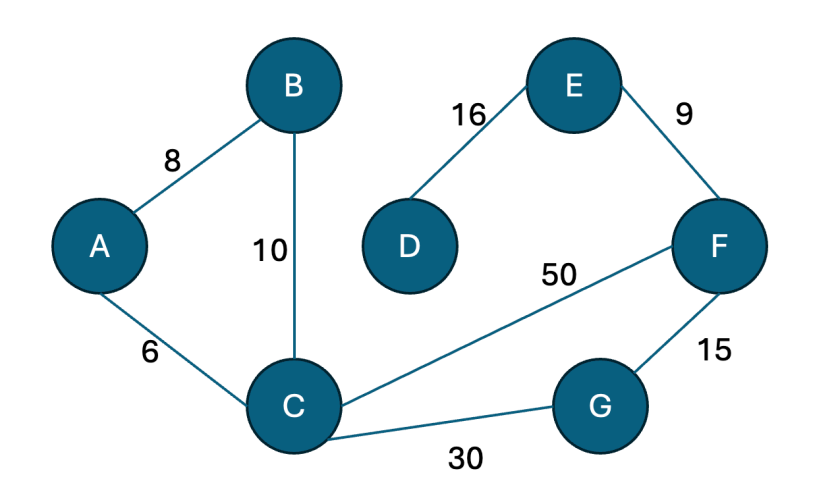
\includegraphics[width=0.6\textwidth]{task1.png} % 插入图片,设置宽度为文本宽度的一半
        % \caption{示例图片} % 图片的标题
        \label{fig:example} % 图片的标签,用于引用
    \end{figure}

    \subsection*{Task 1.1}
    From the BFS algorithm, we can get the path from point A to point D as: \textbf{A, C, F, E, D},\[\text{cost} = 6 + 50 + 9 + 16 = 81 \]

    \subsection*{Task 1.2}
    From the DFS algorithm, we can get the path from point A to point D as:\textbf{A, C, G, F, E, D},\[\text{cost} = 6 + 30 + 15 + 9 + 16 = 76 \]

    \subsection*{Task 1.3}
    From the UCS algorithm, we can get the path from point A to point D as:\textbf{A, C, G, F, E, D},\[\text{cost} = 6 + 30 + 15 + 9 + 16 = 76 \]

    \newpage
    \section*{Problem 2}
    \begin{figure}[h]
        \centering
        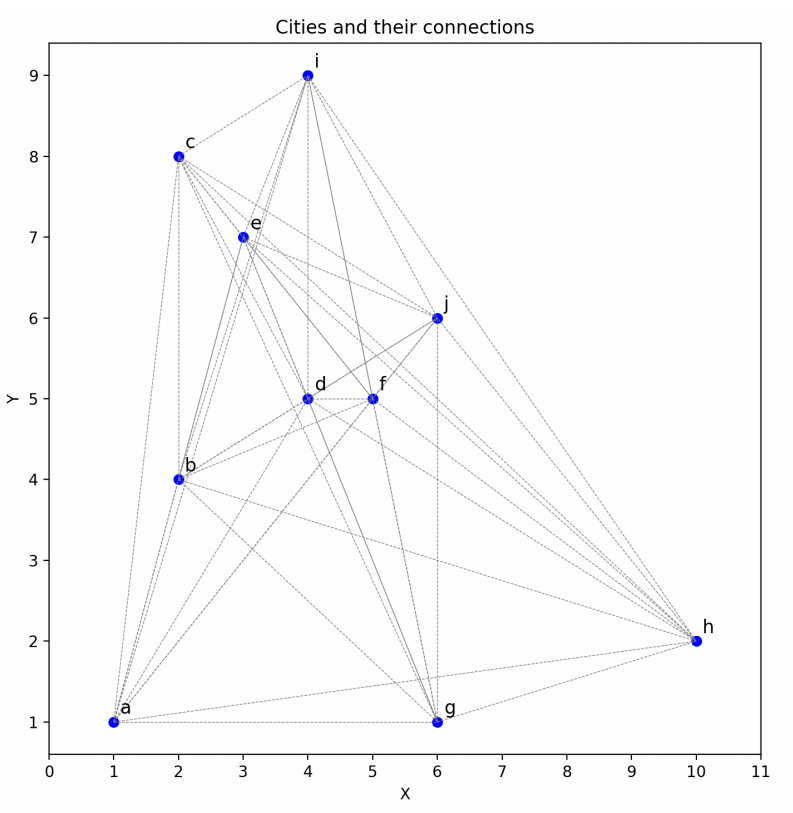
\includegraphics[width=0.6\textwidth]{task2.png} % 插入图片,设置宽度为文本宽度的一半
        % \caption{示例图片} % 图片的标题
        \label{fig:example} % 图片的标签,用于引用
    \end{figure}

    \subsection*{Task 2.1}
    According to the Euclidean distance formula, the distance between the two cities is:
    \[ D_{ij} = \sqrt{(x_i - x_j)^2 + (y_i - y_j)^2} \]
    The goal is to find the shortest path that passes through all cities, and each city can only be visited once.
    Therefore, the mathematical expression can be established: the optimal path\(R = (p_0, p_1, \cdots, p_{n-1})\): 
    \[\min f(R) = \sum_{p = 1}^{n - 1} D_{p, p+1}\]
    where \(n\) represents the number of cities and \(p\) represents the city. The constraints are
    \begin{itemize}
        \item Each city must be visited once.
        \item Must pass through all cities.
    \end{itemize}

    \subsection*{Task 2.2}
    According to task 2.1, we can get\[ \text{the cost of the 'abcdefghij' path} = \sum D_{ij} = 36.904 \]
    \[ \text{the cost of the 'afhbecgijd' path} = \sum D_{ij} = 46.46 \]

    \subsection*{Task 2.3}
    In genetic algorithms, the fitness function is used to measure the quality of a path. For the TSP problem, the fitness function should be inversely proportional to the total length of the path. The shorter the path, the higher the fitness. Therefore, the fitness function can be expressed as:
    \[
    F(R) = \frac{1}{\text{total path length}}
    \]
    Where \( F(R) \) is the fitness of path \( R \), and the total path length is obtained by calculating the sum of the distances between all cities.
    As the path decreases, the fitness increases, and this characteristic guides the algorithm to gradually converge to the optimal path. Therefore, this fitness function can be proven to be effective.
    
    \subsection*{Task 2.4}
    \begin{itemize}
        \item step 1: Get two parent chromosomes \\
        parent path 1 'abcdefghij' \\
        parent path 2 'afhbecgijd'
        \item step 2: Crossover of chromosomes, where the positions of the two crossover points are x: 012x34567x89
        \item step 3: Get offspring paths \\
        offspring path 1 'abc\textcolor{red}{becgi}ij' \\
        offspring path 2 'afh\textcolor{red}{defgh}jd'
        \item step 4: Solve the conflict problem of encoding duplication: According to the mapping b-d, e-e, f-c, g-g, h-i, we can get \\
        offspring path 1: 'adfbecgihj' \\
        offspring path 2: 'acidefghjb'
        \item For code implementation, please check the `DongJunbo12432995.ipynb`
    \end{itemize}

    \subsection*{Task 2.5}
    For the TSP problem, each individual represents a path (i.e., the order of visiting cities), and the mutation operation can introduce new solutions by changing the order of cities in the path. Based on this, the mutation strategy can be designed to randomly exchange two points except the starting point and the end point. The advantage of this design is that it can introduce new city arrangements and explore more path combinations, which can prevent falling into local optimal solutions during the solution process. Compared with the crossover operation, mutation can break some local optimal solutions. At the same time, the mutation strategy requires more solution time than the crossover strategy because the mutation is random, while the crossover strategy can find the optimal solution near the known solution space more quickly.
\end{document}